%==============================================================================
\section{Results}
\label{sec:results}

\subsection{Corpus and structure}
\label{sec:res-corpus}

After the 14 ambient species are folded into the medium, the graph has 5{,}330 internal species and 2{,}914 junctions.
Of the species, 4{,}014 are participants only, 724 modifiers only and 589 both.
The stoichiometric matrix has rank 2{,}667, so the node laws carry 2{,}663 conservation laws and 247 steady flux modes.
The rank cut fell in a clean gap: the smallest kept relative singular value is $1.1\times10^{-5}$ and the largest dropped one $8.9\times10^{-16}$.

With only the medium open, 2{,}364 of the 2{,}914 junctions are blocked (\cref{prop:blocked}): they carry zero flux in every steady state, whatever the rate constants.
When the 4{,}002 boundary species, those that are only produced or only consumed, are also opened, 95 junctions remain blocked.
The difference is a structural statement about the curated corpus.
Most cytosolic reactions are fragments of pathways whose other steps lie outside the cytosol or outside Reactome's cytosolic annotations, and they can carry flux only if their boundary species are exchanged.

No node value is solved.
For 4{,}603 species the solve is \vd{absent}; for 4{,}568 of them rate constants, equilibrium constants and concentrations are all missing.
The other 727 are \vd{underdetermined}: modifiers whose node law is $0=0$.
No solve is the expected result for a kernel that refuses to supply parameters, and it fixes the baseline against which every later stage is measured.

\paragraph{Cut keys and refinement.}
At radius 1, the local separation cost takes 41 distinct values and the cut key 63, with $\sigma_1\le288$, $\delta_1\le14$ and balls of up to 135 items.
At radius 2 the cut key takes 64 values.
Colour refinement from the radius-1 key proceeds through nine partitions, every one refining the last (\cref{fig:refinement}), and ends with 6{,}792 classes over 8{,}244 items.
Of the junctions, 2{,}524 classes remain and 537 junctions share a class; the largest shared class has 71 members, all binding events (for example, 14-3-3 proteins binding phosphorylated forkhead box proteins).
Locating an item within its class needs 0.65 bits on average and at most 7.1 bits.
With 63 initial key values, at least $\log 8244/\log 63 = 2.2$ independent keys are needed to give every item a distinct position.

\begin{figure}[t]
\centering
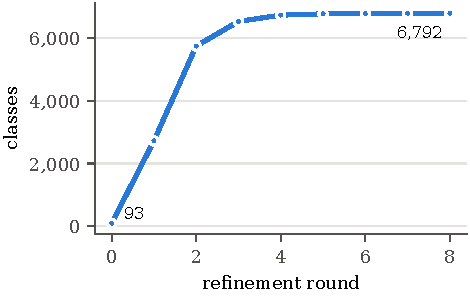
\includegraphics[width=0.48\linewidth]{figures/refinement.pdf}
\caption{Colour refinement from the radius-1 cut key.
Each round refines the previous partition (\cref{prop:refine}); the number of classes grows from 93 to 6{,}792 and then stops.
The 1{,}988 items left in shared classes are structurally indistinguishable at any depth.}
\label{fig:refinement}
\end{figure}

\paragraph{Ladders.}
The graph contains 17 maximal unbranched series chains.
The longest has ten rungs: the steps of retroviral reverse transcription, from RNase H cleavage of the RNA strand to synthesis of full-length duplex DNA.
Every chain's rung powers are \vd{absent}, with the blocker ``rung power needs junction conductances'': without conductances, \cref{prop:ladder} cannot be evaluated.

\subsection{Thermodynamic coverage}
\label{sec:res-thermo}

TECRDB contributes 418 reactions in the temperature and grade window, 295 of them with a transformed value in the pH window.
Matching gives 75 kernel reactions with a measured $\DG$, all via \conv{conjugate-closure} (71), a candidate selected by the TECRDB match (3) or water balance (1).
They correspond to 61 distinct TECRDB reactions.
Of the rest, 2{,}244 are \vd{refused} because a participant is a macromolecule, and 595 are \vd{absent}.
Of the absent, 398 have no TECRDB measurement and 197 have a participant without a KEGG identifier (\cref{fig:coverage}).

\begin{figure}[t]
\centering
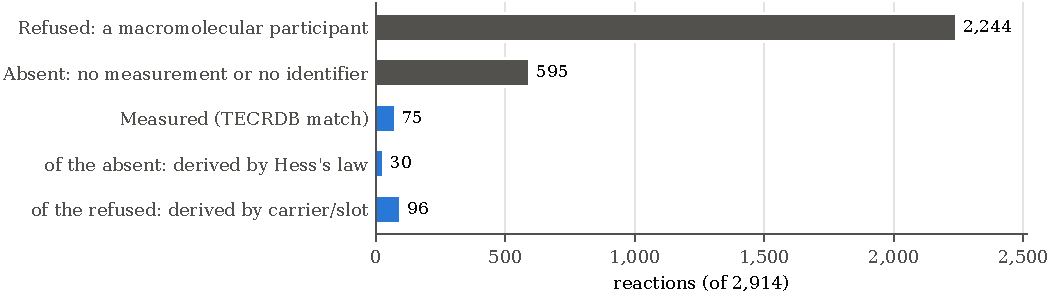
\includegraphics[width=0.85\linewidth]{figures/coverage.pdf}
\caption{Thermodynamic verdicts for the 2{,}914 cytosolic reactions.
Grey bars partition the reactions that TECRDB does not determine directly; blue bars are the reactions with a chemical-reference $\DG$.
Hess's law recovers 30 of the absent and the carrier/slot decomposition 96 of the refused.}
\label{fig:coverage}
\end{figure}

\paragraph{Cycle consistency.}
The 61 distinct matched reactions are linearly independent: $\ker S$ is trivial, and the cycle test is \vd{certified-empty}.
The question is well posed and its answer is empty, because the kernel's measured reactions close no cycle.
The full TECRDB set is not internally consistent.
The weighted Hess fit over 418 reactions and 495 compounds has $\chi^2=275.6$ on 67 degrees of freedom ($\chi^2/\nu=4.11$, Birge ratio 2.03), so the quoted uncertainties are about half the scatter they must explain.

\paragraph{Hess's law.}
Of 398 small-molecule reactions that TECRDB never measured directly, 30 lie in the span of the measured reactions and are \vd{answered} (\cref{prop:hess}).
One is \vd{certified-empty} (no net chemical change).
The other 367 are \vd{absent}: 324 contain a compound never measured in any TECRDB reaction, and 43 are not combinations of measured reactions.

\paragraph{Carrier and slot.}
Of the 2{,}244 refused reactions, 1{,}591 are not carrier reactions, because the protein entity differs between the two sides.
Of the remaining 653, 96 are \vd{answered} (94 kinase and 2 phosphatase steps) and 104 are \vd{underdetermined}, because the species names state a number of changed sites that does not match the number of kinase or phosphatase steps.
The other 453 are \vd{absent}: 373 involve carrier chemistry other than phosphoryl transfer, and 80 a compound that TECRDB never measured.

\paragraph{Enzyme expansion.}
Expanding the 1{,}116 catalysts into two-rung cycles gives 4{,}546 junctions over 6{,}962 species, with rank 4{,}299.
The conservation-law dimension stays 2{,}663 and the flux-mode dimension 247, as \cref{prop:enzyme} requires of an expansion that leaves net stoichiometries unchanged.
The enzyme total is conserved for 682 catalysts and broken for 434, which the stoichiometry also makes, consumes or modifies.

\paragraph{Direction in the base stage.}
With TECRDB's transformed study means in the pH window and the 1\,\textmu M--10\,mM concentration window, 3 reactions are \vd{answered} forward and 61 are \vd{undecidable}.
The remainder inherit \vd{absent} (606) or \vd{refused} (2{,}244) from the match.

\subsection{Proteins and attachment}
\label{sec:res-proteins}

Of the phosphosites named on carrier reactions, 206 were located in their protein's sequence with the named residue type.
Another 69 named no position, 9 named a residue type that differs from the sequence, 12 belong to proteins without an AlphaFold contact graph and 35 to an entity whose protein was not determined.
The located sites lie on 131 reactions and 101 proteins; attaching them adds 60{,}657 residue vertices, 222{,}072 contact edges and 206 slot edges.

\paragraph{Monotonicity and its control.}
Over the 60 items whose global separation cost was computed before and after attachment, attachment never lowered $\sigma$ (0 decreases, 20 increases), as \cref{prop:monotone} requires.
The control replaced each carrier--junction edge's counted weight by the slot residue's relative exposure, a real number in $(0,1]$.
It lowered $\sigma$ for 46 of the 60 items and raised it for 4, and the minimum fell from 2 to 1.14.
Local separation costs at radii 1 and 2 behave the same way under attachment: of 423 items, none decreased and 131 increased.

\paragraph{Exposure of phosphosites.}
Named sites are more exposed than residues of the same type in the same proteins (one-sided Mann--Whitney $p=0.0049$; 165 sites against 4{,}443 residues).
The medians are equal (5 exposed heavy atoms each), and the difference is at the bottom of the distribution: no named site is buried, against 3.1\% of the comparison residues.

\subsection{The medium as eluent (M1--M3)}
\label{sec:res-medium}

\paragraph{The transform.}
Our Legendre transform reproduces eQuilibrator's own transform on all 3{,}276 TECRDB rows in the window, with a largest difference of $6.8\times10^{-13}\kJ$.
Two controls confirm that the comparison can fail: shifting the pH by 0.1 leaves only 66 rows within $10^{-6}\kJ$, and dropping the Debye--H\"uckel term leaves 59.

\paragraph{M1: the medium transfers (supported).}
For TECRDB reactions measured under three or more distinct conditions, each condition was held out in turn and predicted from the others.
The \emph{medium} model fits one chemical-reference value per reaction and adds the held-out row's transform.
The \emph{constant} model predicts the training mean, and the \emph{affine-pH} model fits a line in pH (two parameters).
Replicate noise, the same reaction under the same conditions in different studies, is 1.38\kJ\ in mean (0.71 median) over 171 pairs.
\Cref{fig:transfer} gives the errors.
Paired per reaction, the medium model beats the constant model in 84 of 137 interpolated reactions (Wilcoxon $p=8\times10^{-4}$) and in 95 of 154 extrapolated ones ($p=5\times10^{-6}$).
Where the held-out transform moved by more than 1\kJ, the interpolation errors are 1.95 against 2.94\kJ; where it moved less, they are equal (1.08 and 1.08).
The medium model's mean error is 1.13 times the replicate noise in interpolation and 1.88 times in extrapolation, within the stated limit of twice the noise.
In extrapolation it is no worse than affine-pH (82 against 72 reactions, $p=0.27$).
One result was not predicted: in interpolation, the two-parameter affine-pH model beats the one-parameter medium model (77 against 58 reactions, $p=0.009$).

\begin{figure}[t]
\centering
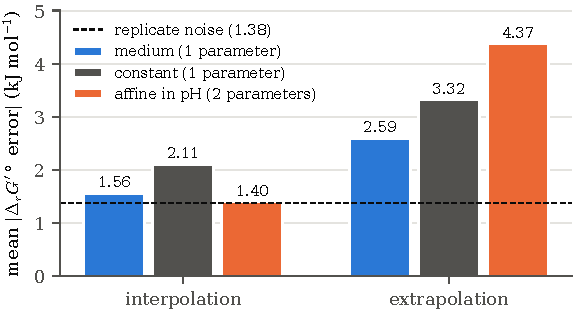
\includegraphics[width=0.62\linewidth]{figures/transfer.pdf}
\caption{Held-out prediction of transformed Gibbs energies (M1).
Mean absolute error over held-out TECRDB rows for three models.
The dashed line is the replicate noise between studies of the same reaction under the same conditions.}
\label{fig:transfer}
\end{figure}

\paragraph{M2: direction (count fails, attribution holds).}
Of the 201 reactions with a chemical value, 2 are \vd{answered} forward: pyrophosphate hydrolysis by the two cytosolic pyrophosphatases.
The claim of more than three answered fails.
The base stage's three answers used study means without uncertainty or ionic-strength and magnesium ranges.
Adding $q\sigma$ and those ranges removes one of them, AMP hydrolysis by a nucleotidase, which rested on a single study.
The two survivors clear zero by only 0.28\kJ.
The second part holds: of the 199 undecided reactions, 156 (78\%) have a fixed sign of $\DGm$ across the medium window, including all 96 carrier/slot reactions.
For these, the concentrations, not the medium, are what remain to be measured; the other 43 are blocked by the medium window itself.

\paragraph{M3: crowding and dilution (both fail).}
Crowding changes both of the two decided verdicts, far above the stated limit of 5\%.
In each pyrophosphate hydrolysis, one pyrophosphate and one water give two phosphates, so with water excluded the reaction adds one solute particle.
Its 0.28\kJ\ margin is below the 0.92\kJ\ crowding shift at $a=0.7$.
With crowding in the medium, no reaction in the kernel has a decided direction.
The dilute-solution bound $2nv$, with $n$ the number density at 10\,mM and $v$ the molecular volume, has a median of 0.0035 per particle but exceeds $10^{-2}$ for large compounds.
The worst is a 1{,}873\,Da compound (KEGG C05893) at 0.027.
The ideal-solution form of $\mu$ is safe for ordinary metabolites at 10\,mM, but not for molecules of this size at the top of the window.
A hard-sphere second-virial estimate would give a larger factor than $2nv$, which would strengthen this failure rather than remove it.

\subsection{Kinetics: retention, locality and K1}
\label{sec:res-kinetics}

SABIO-RK's 7{,}458 human wild-type entries with $K_m$ give 5{,}682 substrate $K_m$ records over 3{,}559 (protein, compound) pairs.

\paragraph{Retention.}
370 of the 1{,}631 catalysed kernel reactions have a measured $K_m$ for a substrate, giving 596 contacts.
Of 168 metabolites with a $K_m$, 161 have a PaxDb abundance for every binding enzyme.
Their median retention factor at total enzyme is 0.001--0.003 across the 2--6\,mM range of total protein, so metabolites are almost entirely free and binding barely raises their capacitance.
Only 8 exceed $k=1$ at the upper total, among them 5-diphosphoinositol pentakisphosphate ($k=9$--26), S-adenosylmethionine, fructose 1,6-bisphosphate and NADPH.

\paragraph{Locality.}
The enzymes are not dilute.
Over 223 enzymes, the median concentration $c^\ast$ at which the readout departs by 10\% from the dilute limit is 2.4\,\textmu M of substrate.
Of these enzymes, 76 depart below 1\,\textmu M of substrate.
None stays dilute across the whole concentration window, and 221 depart by more than 10\% at 1\,mM.
106 enzymes have two or more measured substrates that share the same sites.
In chromatographic terms the cytosolic column is overloaded.
For the metabolite the stationary phase is negligible ($k\ll1$), but for the enzyme the contacts are non-local (Langmuir rather than linear).
Enzyme--substrate states therefore cannot be folded into the free species' capacitance; they must stay explicit with conserved enzyme totals, as in \cref{sec:enzyme}.

\paragraph{K1: whole-protein descriptors do not carry $K_m$ (holds).}
Under leave-one-protein-out cross-validation over 272 proteins and 1{,}228 pairs, the baseline predicts each $K_m$ from the substrate's mean $\log_{10}K_m$ over other proteins.
The alternative adds a ridge map from five AlphaFold descriptors to the residual: residue count, mean pLDDT, fraction of buried residues, mean contact weight per residue and exposed atoms per residue.
Its ridge penalty is chosen by inner five-fold cross-validation.
The mean absolute errors are 0.775 and 0.780 $\log_{10}$ units.
The descriptor model is better for 105 proteins and worse for 127 (one-sided Wilcoxon $p=0.94$), so the claim that descriptors do not help holds.
The positive control adds a synthetic effect of 0.5 standard deviations of $\log_{10}$(residue count) to $\log_{10}K_m$; the test detects it ($p=0.007$), so it could have found an effect that the descriptors carry.

\subsection{Completion and separation}
\label{sec:res-complete}

The survey asks, for 540 small-molecule sources and 779 targets (420{,}120 pairs), whether the kernel turns the source into the target using only the source, the medium and the 2{,}241 proteins that no reaction makes.
\Cref{fig:completion} gives the outcomes under the three direction semantics.

\begin{figure}[t]
\centering
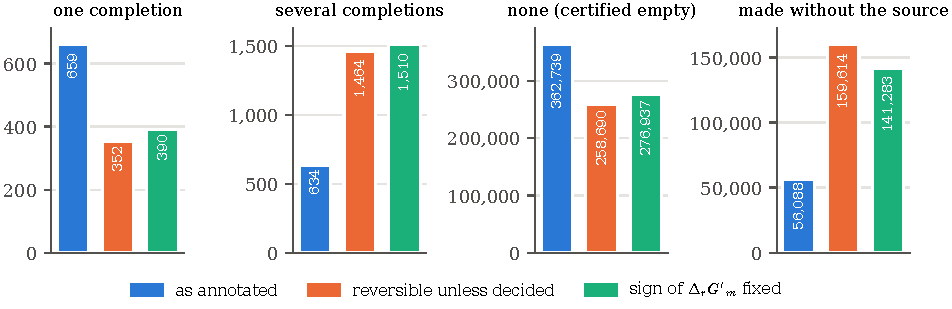
\includegraphics[width=\linewidth]{figures/completion.pdf}
\caption{Completion outcomes for 420{,}120 source--target pairs under three direction semantics.
Each panel has its own scale.
``Made without the source'' means the target is reached from the medium and proteins alone.}
\label{fig:completion}
\end{figure}

Most pairs have no completion, because most reactions need a second small molecule that a single source cannot supply.
Allowing reactions to run backwards halves the unique completions, from 659 to 352.
It also lets the medium and proteins make many more targets on their own (56{,}088 to 159{,}614).
Fixing the 158 directions whose $\DGm$ sign is fixed (two by measurement and 156 by the 1\,mM sign) adds 38 unique completions (+11\%) and removes 18{,}331 pairs from ``made without the source''.
A completion may not pass through its own target, but alternatives through other cycles among intermediates still count as several, so that column is an upper count.

\subsection{A coupled-oscillator account of folding (F1--F5)}
\label{sec:res-folding}

We tested an account of folding in which residues are phase oscillators coupled by a matrix $K$, secondary structure emerges as groups of phase-locked residues, and the number of large eigenvalues of $K$ counts secondary-structure elements.
The account is a variant of Kuramoto synchronisation \citep{kuramoto1984chemical} and is motivated by Levinthal's argument that folding cannot be an unbiased search \citep{levinthal1969fold,dill2012folding}.
Its coupling is built from sequence alone ($K_{\mathrm{seq}}$).
We also ran every test with the AlphaFold contact graph as coupling ($K_{\mathrm{AF}}$, counted heavy-atom pairs within 4.5\,\AA), which gives the account the real structure to work with.
Secondary-structure elements come from a backbone hydrogen-bond assignment in the manner of \citet{kabsch1983dssp}.
Against the authors' helix and sheet records in four experimental structures, that assignment agrees per residue at 0.87 (1CRN), 0.83 (1UBQ), 0.87 (2LZM) and 0.91 (3CHY), against 0.24--0.42 for shuffled residues.

\paragraph{F1: contacts from sequence (reproduction).}
On 607 AlphaFold models with mean pLDDT at least 90 and 50--400 residues, $K_{\mathrm{seq}}$ reaches a top-$L$ contact precision of 0.81 times the base rate, worse than random (two-sided Wilcoxon $p=7\times10^{-11}$).
A plain hydrophobicity product reaches 2.36 times the base rate.
No protein meets a criterion of precision at least 0.7 and recall at least 0.5 with either score.

\paragraph{F2: eigenvalue count equals the number of elements (fails).}
On 149 proteins with a median of 12 elements, no protein's count of $K_{\mathrm{seq}}$ eigenvalues above the threshold matches exactly, with a mean absolute error of 7.1; $K_{\mathrm{AF}}$ matches 3, with error 9.1.
A baseline that predicts the count from length alone matches 23, with error 2.2.
Both couplings give too many eigenvalues above threshold (medians 18 and 20), even $K_{\mathrm{AF}}$, which is built from the real structure.

\paragraph{F3: phase-lock groups are secondary structure (fails).}
Agreement with the element/loop segmentation, as the best adjusted Rand index over a sweep of coupling strengths, is 0.067 for $K_{\mathrm{AF}}$ phase-lock groups.
Equal contiguous blocks score 0.486 and win for 148 of 149 proteins.
$K_{\mathrm{seq}}$ groups score 0.001.
The dynamics also add nothing to the coupling they run on: the connected components of the top $K_{\mathrm{AF}}$ pairs score 0.057, and the dynamics win 80 proteins and lose 66 ($p=0.14$).

\paragraph{F4: phosphosites are less synchronised, and disorder accounts for it (both parts hold, the second weakly).}
Kuramoto dynamics on $K_{\mathrm{AF}}$ at a coupling of 2, fixed in advance, give each residue a local order parameter.
Over 158 located sites against 3{,}870 same-type residues, sites have lower local order (median 0.912 against 0.936, one-sided $p=0.012$) and lower pLDDT (53.7 against 57.9, $p=0.043$).
Within pLDDT strata the difference is not significant: $p=0.39$ below 70 (106 sites) and $p=0.13$ at 70 or above (52 sites).
The second part rests on an absence of significance in a small stratum whose medians still point the same way (0.933 against 0.953), so a small residual effect is not excluded.
D1 (\cref{sec:res-db}) returns to this with measured disorder.

\paragraph{F5: hierarchical ternary addresses (measurement).}
C$\alpha$ coordinates normalised to each protein's bounding cube were given interleaved base-3 addresses.
On 150 models, the distance-preservation bound holds for all 2{,}480{,}054 C$\alpha$ pairs.
The deepest level whose cells are at least 8\,\AA\ on a side is one full triple of digits (27 cells), and only 54.6\% of the 122{,}559 C$\alpha$ contacts share that prefix.
The address bounds distance when prefixes agree but misses 45\% of contacts that straddle a cell boundary; it is usable as a proximity key only together with neighbouring cells.

\subsection{Verdict axes and extensions (E1--E6)}
\label{sec:res-extend}

The extension stage used every human wild-type kinetic law in SABIO-RK, UniProt annotations for 3{,}207 proteins (1{,}481 with an EC number) and PaxDb abundances for 3{,}048 proteins.

\paragraph{E1: verdict axes (measurement).}
Every empty or absent verdict from the live producers carries a gate letter.
These producers are the thermodynamic match, Hess, carrier/slot, direction, modifiers, dividers, variants and the redox ladder.
Of 1{,}681 such verdicts, 686 are not recorded ($-$), 605 are a name the source never uses (\textsf{open}) and 390 are witnessed absent ($+$); none is undecided.
The ground verdicts of each fact family are those given in \cref{sec:ground}.
The stage digest is current under its own conventions and stale after a change of pH window.
On the specification example, \vd{subfloor} reproduces a composite of 0.9475 against a target of 0.95, a shortfall of 0.0025.
On real data, no ladder chain has all its rung conductances (0 of 17), so it never fires.

\paragraph{E2: modifiers (measurement).}
Of 175 inhibitor edges, 147 are macromolecular partners and \vd{refused}; 26 small molecules have no $K_i$ for their enzyme in SABIO-RK ($-$) and 2 have no KEGG compound (\textsf{open}).
Of 105 stimulator edges, 52 are macromolecular, and the 53 small molecules have no activation constant.
No modifier edge is answered.
The 434 broken enzyme totals arise from assembly or dissociation (266), covalent modification (140), degradation (124) and other reactions (103); an enzyme may have several kinds, and where only one applies the counts are 91, 52, 49 and 45.
Such reactions are the boundary currents through which induction and inactivation would act.
Of 58 loss-of-function variant reactions, 23 attach to a single wild-type edge as a modifier, 19 match several (\vd{underdetermined}) and 16 match none.

\paragraph{E3: flux dividers (measurement).}
Of 168 branch points in healthy cells, 3 are \vd{answered}; the others lack $k_{\mathrm{cat}}/K_m$ for a sibling (487 sibling gaps) or have an uncatalysed sibling (135).
On average 7.6\% of a branch point's siblings are complete.
The answered shares are: fructose 1,6-bisphosphate to fructose-1,6-bisphosphatase 0.67 and aldolase 0.33; galactose to galactokinase 0.98 and aldose reductase 0.02; glucose to aldose reductase 0.52 and hexokinases 0.48.
The glucose share is not credible.
At millimolar glucose the hexokinases are saturated ($K_m$ about 0.1\,mM), so the dilute limit does not hold; this repeats the locality failure of \cref{sec:res-kinetics}.

\paragraph{E4: the redox ladder (E4a, E4b hold; E4c untestable).}
\Cref{tab:redox} gives the couple potentials derived from the Hess span.
The NAD and NADP couples lie 1.6\,mV apart, within the predicted 10\,mV (E4a).
With glutathione disulfide (GSSG) and reduced glutathione (GSH), NADPH + GSSG $\to$ NADP$^+$ + 2\,GSH has $\DGp=-13.8\kJ$, inside the predicted $-16\pm10\kJ$ (E4b).
Cystine and dehydroascorbate were never measured in TECRDB (\textsf{open}), and flavin adenine dinucleotide is not a combination of measured reactions ($-$).
For E4c, the flavin-to-cysteine edge distance is 3.42\,\AA\ in glutathione reductase (Protein Data Bank (PDB) entry 3GRS) and 3.33\,\AA\ in thioredoxin reductase 1 (2J3N).
Both give a ruler rate of $6.8\times10^{10}\,\mathrm{s^{-1}}$, and the control at 25\,\AA\ gives $0.014\,\mathrm{s^{-1}}$, so the check could discriminate.
SABIO-RK has no human wild-type $k_{\mathrm{cat}}$ for either enzyme, so E4c is \vd{absent} and untested.

\begin{table}[t]
\centering
\caption{Redox couples derived from the Hess span at pH 7, $I=0.25$\,M, 298.15\,K, relative to NADP$^+$/NADPH.
Textbook differences are approximate.}
\label{tab:redox}
\small
\begin{tabular}{@{}lrrr@{}}
\toprule
Couple & $E-E_{\mathrm{NADP}}$ (mV) & $\sigma$ (mV) & Textbook difference (mV) \\
\midrule
NAD$^+$/NADH & $+1.6$ & 7.5 & $+4$ \\
GSSG/GSH & $+71.7$ & 12.7 & about $+84$ \\
lipoamide & $+25.1$ & 29.1 & about $+34$ \\
thioredoxin & $+57.9$ & 28.2 & about $+54$ \\
pyruvate/lactate & $+138.7$ & 10.6 & $+139$ \\
oxaloacetate/malate & $+156.6$ & 9.1 & $+158$ \\
\bottomrule
\end{tabular}
\end{table}

\paragraph{E5: EC labels are concordant with structural classes (holds).}
Real level-1 EC labels split 4 of the 147 shared junction classes that carry labels (210 labelled junctions).
Shuffled labels split 53.7 on average, with a minimum of 41 (empirical $p=0.005$); at level 3 the counts are 4 against 61.8.
For 100 classes no label splits them (\vd{underdetermined}).
For the rest, the coarsest splitting label is the gene (18), EC level 1 (11), Pfam (8), EC level 4 (8), EC level 2 (1) or EC level 3 (1), and 32 classes are separated completely.
The bits left per item fall from 0.649 with structure alone to 0.641 with EC level 1, 0.629 with EC level 4, 0.627 with Pfam and 0.619 with the gene.

\paragraph{E6: stoichiometric signatures match EC classes (holds).}
The signature rules give 798 \vd{answered}, 42 \vd{underdetermined} (28 of them lyase and transferase together), 653 \vd{absent} and 1{,}421 \vd{refused} verdicts.
On 634 reactions with a single-class catalyst, the signature agrees with the EC class in 593 (93.5\%), against 32.5\% for shuffled labels (empirical $p=0.005$).
The largest confusions are lyase against EC oxidoreductase (8) and hydrolase against EC transferase (8).

\subsection{Cross-checks against curated databases (R1--G1)}
\label{sec:res-db}

\paragraph{R1: curated direction against the 1\,mM sign (fails).}
460 kernel reactions map to Rhea (403 left-to-right, 69 right-to-left), and their participant sets agree in 421 of 459.
For the 62 mapped reactions whose $\DGm$ sign is fixed across the medium window, the sign agrees with the curated direction in 45 (72.6\%), below the predicted 80\%.
The 17 disagreements are not errors of sign.
They include triose-phosphate isomerase, glyceraldehyde-3-phosphate dehydrogenase, lactate oxidation by lactate dehydrogenase, ethanol oxidation, creatine kinase forming phosphocreatine and the thiolase condensation of two acetyl-CoA.
All of them run uphill at 1\,mM and proceed in the cell because product is drawn away.
The 1\,mM sign is not a direction; the concentration ratio is.
Measured concentration windows (\cref{sec:loaders}) would decide exactly these reactions.

\paragraph{I1: MetaNetX closes identifier misses (fails).}
MetaNetX gives 36 more species a KEGG compound and unblocks 34 of the 197 reactions blocked by a missing identifier (17\%, against a predicted quarter).
One of them gains a TECRDB match, and 33 are now blocked by ``no TECRDB measurement of this reaction''; the Hess-derived count stays at 30.
The gate letter of those 33 changes from \textsf{open} to $-$: the limit is measurement, not identifiers.

\paragraph{L1: catalysts have cytosol support (holds).}
Of 2{,}134 catalyst proteins, 1{,}947 have cytosol support, 100 have none and 87 have no data, so 95.1\% of those with data are supported.
By reaction, 1{,}404 have all catalysts supported, 79 some and 78 none.
The unsupported proteins include the three fibrinogen chains (UniProt P02671, P02675 and P02679), which are secreted.
The 78 reactions are candidates for errors in the cytosol annotation from which the corpus was filtered.

\paragraph{S1: slots sit on curated phospho-residues (holds).}
168 of the 206 located phosphosites (81.6\%) coincide with a UniProt phospho modified residue.
141 of the 168 carry experimental evidence (ECO:0000269 or ECO:0007744).
One numbering offset per protein explains 5 of the 9 residue mismatches: $+39$ in Q04637 (3 sites), $+2$ in Q14155 and $-48$ in tau (P10636, an isoform numbering).
UniProt also names 31 phosphorylated enzyme intermediates (phosphohistidine, phosphocysteine, phosphoserine) among the catalysts; these are the enzymes whose two-rung expansion should carry a covalent intermediate.
A first run reported 19\%: the parser cut each UniProt note at its first semicolon, losing notes such as ``Phosphoserine; by MTOR'' that name the kinase, here the mechanistic target of rapamycin (MTOR).
The corrected parser has a regression test.

\paragraph{C1: catalytic residues are contact hubs (holds).}
Over 50 M-CSA enzymes, 255 catalytic residues have a median of 55 heavy-atom contacts, against 43 for the 3{,}773 residues of the same amino-acid types in the same AlphaFold models (one-sided Mann--Whitney $p=2.7\times10^{-18}$).
A random same-type sample of equal size gives $p=0.46$.

\paragraph{A1: AlphaFold contacts match experiment (holds).}
Of 313 high-confidence models, 60 were compared with an experimental chain (\cref{fig:structures}).
The median Jaccard index of contact sets is 0.90; shifting one numbering by three residues drops it to 0.14.
Buried and exposed calls agree for 95\% of residues.
On these proteins, the AlphaFold contact graphs used for attachment and for F1--F5 stand in for measured ones.

\begin{figure}[t]
\centering
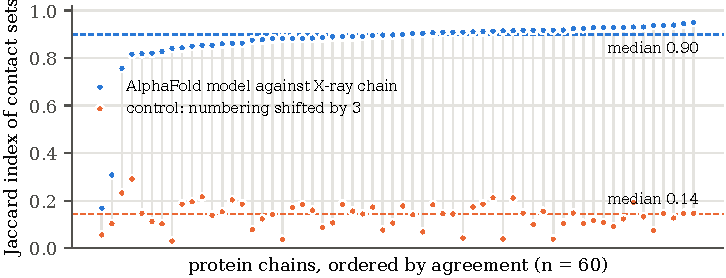
\includegraphics[width=0.85\linewidth]{figures/structures.pdf}
\caption{Contact agreement between AlphaFold models and X-ray chains for 60 proteins (A1).
Blue: Jaccard index of residue contact sets.
Orange: the same after shifting one numbering by three residues.
Dashed lines are medians.}
\label{fig:structures}
\end{figure}

\paragraph{D1: measured disorder explains the phosphosite effect (fails).}
Over 40 proteins with located sites and DisProt entries, named sites outside the disordered regions still have lower local order than same-type residues (median 0.88 against 0.94, one-sided $p=0.0012$, 34 sites).
Inside disordered regions they do not differ ($p=0.37$, 26 sites).
Measured disorder does not account for the effect that pLDDT appeared to account for in F4.
DisProt is incomplete, so ``outside a DisProt region'' is not the same as ``ordered''.

\paragraph{G1: Human-GEM coefficients agree (holds, weakly discriminating).}
505 kernel small-molecule reactions have KEGG identifiers for every participant; 324 match a Human-GEM cytosolic reaction by participant set, and all 324 have the same coefficients.
Only 23 of them have a coefficient other than 1, so the agreement rests on those 23.
Reversibility agrees in 244 of 324.

\paragraph{Per-cell-type abundance.}
With HeLa abundances \citep{nagaraj2011hela} in place of whole-organism ones, 1 branch point is answered instead of 3; galactose goes to galactokinase with share 0.96, against 0.98.

\subsection{Summary of outcomes}
\label{sec:res-summary}

\Cref{tab:outcomes} lists the 23 pre-registered claims.
Fourteen held, eight failed and one could not be tested.

\begin{table}[p]
\centering
\caption{Outcomes of the 23 pre-registered claims.}
\label{tab:outcomes}
\small
\begin{tabularx}{\linewidth}{@{}l>{\raggedright\arraybackslash}Xl>{\raggedright\arraybackslash}p{4.6cm}@{}}
\toprule
ID & Claim & Outcome & Key number \\
\midrule
M1 & the medium transform transfers between conditions & holds & error 1.13$\times$ (interp.) and 1.88$\times$ (extrap.) replicate noise \\
M2a & more than 3 reactions get a direction & fails & 2 answered \\
M2b & concentrations, not the medium, block most of the rest & holds & 156 of 199 \\
M3a & crowding changes at most 5\% of decided verdicts & fails & 2 of 2 changed \\
M3b & dilute bound below $10^{-2}$ for every metabolite at 10\,mM & fails & worst 0.027 \\
K1 & protein descriptors do not improve $K_m$ prediction & holds & $p=0.94$; positive control $p=0.007$ \\
F2 & eigenvalue count equals number of elements & fails & 0 and 3 exact, against 23 for length \\
F3 & phase-lock groups beat contiguous blocks & fails & 0.067 against 0.486 \\
F4a & phosphosites have lower local order & holds & $p=0.012$ \\
F4b & no difference within pLDDT strata & holds (weak) & $p=0.39$ and $0.13$ \\
E4a & NAD and NADP couples within 10\,mV & holds & 1.6\,mV \\
E4b & NADPH reduces GSSG, $\DGp$ within $-16\pm10\kJ$ & holds & $-13.8\kJ$ \\
E4c & ruler rate exceeds $k_{\mathrm{cat}}$ & untestable & no $k_{\mathrm{cat}}$ in SABIO-RK \\
E5 & EC labels split fewer classes than shuffled labels & holds & 4 against 53.7; $p=0.005$ \\
E6 & signatures agree with EC classes above 60\% and the null & holds & 93.5\% against 32.5\% \\
R1 & 1\,mM sign agrees with curated direction above 80\% & fails & 72.6\% \\
I1 & MetaNetX unblocks at least a quarter of 197 reactions & fails & 34 (17\%) \\
L1 & at least 80\% of catalysts have cytosol support & holds & 95.1\% \\
S1 & at least 70\% of slots on phospho-residues; offsets explain a third of mismatches & holds & 81.6\%; 5 of 9 \\
C1 & catalytic residues have more contacts & holds & $p=2.7\times10^{-18}$; control $p=0.46$ \\
A1 & median contact Jaccard at least 0.6; shifted control below 0.2 & holds & 0.90; 0.14 \\
D1 & outside DisProt disorder, sites do not have lower order & fails & $p=0.0012$ \\
G1 & Human-GEM coefficients agree in at least 90\% & holds & 324 of 324 (23 discriminating) \\
\bottomrule
\end{tabularx}
\end{table}
